\documentclass[10pt]{article}
\usepackage[polish]{babel}
\usepackage[utf8]{inputenc}
\usepackage[T1]{fontenc}
\usepackage{amsmath}
\usepackage{amsfonts}
\usepackage{amssymb}
\usepackage[version=4]{mhchem}
\usepackage{stmaryrd}
\usepackage{graphicx}
\usepackage[export]{adjustbox}
\graphicspath{ {./images/} }

\begin{document}
\begin{enumerate}
  \item Dany jest punkt \(A\), prosta \(k\) oraz okrąg \(\omega\). Skonstruuj takie punkty B i C lezące odpowiednio na prostej \(k\) i okręgu \(\omega\), że trójkąt ABC jest równoboczny. Podaj opis\\
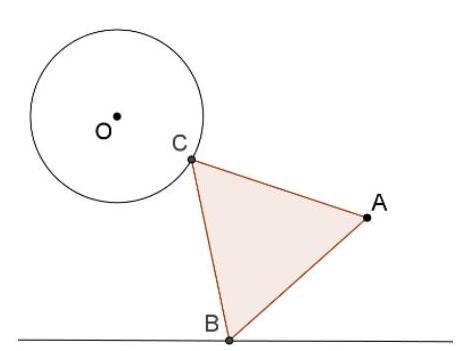
\includegraphics[max width=\textwidth, center]{2024_11_21_08cb668264822452503bg-1}\\
konstrukcji i uzasadnienie jej poprawności. Czy konstrukcja jest zawsze wykonalna?
  \item Wewnątrz trójkąta równobocznego \(A B C\) obrano punkt \(P\) taki, że \(A P=a, B P=b, C P=c\), gdzie \(a^{2}+b^{2}=c^{2}\). Wyznacz miarę kąta APB oraz (dla klasy drugiej) długość boku trójkąta ABC.
  \item Znajdź wszystkie czterocyfrowe palindromy, które mogą być zapisane jako suma dwóch trzycyfrowych palindromów. Palindrom to liczba, która czytana z lewej i prawej strony jest taka sama np. 3017103.
\end{enumerate}

\end{document}